\begin{figure*}[pbt!]
\small
\centering
\begin{tabular}{|p{0.95\linewidth}|} \hline
\begin{minipage}{.45\linewidth}
\small

{\bf \fig{xtree}.A: Top-down division with Decision Trees}

Find a split in the values of independent features (OO metrics) that most reduces the variability
of the dependent feature (defect counts). For continuous and discrete values,
the {\em variability} can be measured using standard deviation $\sigma$ or entropy $e$ respectively. Construct a standard decision tree using these splits.
\\[-0.15cm]
~\hrule~
\\
{\bf \fig{xtree}.B: Finding the most informative nodes}

Discretize all numeric features using the Fayyad-Iranni discretizer~\cite{fi}
(divide numeric columns into bins $B_i$, each of which  select for the fewest cluster ids).
Let feature $F$ have bins $B_i$, each of which contains $n_i$ rows
and 
let each bin $B_i$ have entropy $e_i$ computed from the frequency of clusters seen in that bin.
Cull the the features as per~\cite{papa13}; i.e. just use the $\beta=33\%$ most informative features
where  the   value of  feature $F$ is $\sum_i e_i\frac{n_i}{N}$ ($N$ is the number of rows).\\[-0.1cm]


%   ~\hrule~


% \end{shaded}
\end{minipage}~~~~~\begin{minipage}{.525\linewidth}
% ~\hrule~

\textbf{\fig{xtree}.D: A sample decision tree.\\}
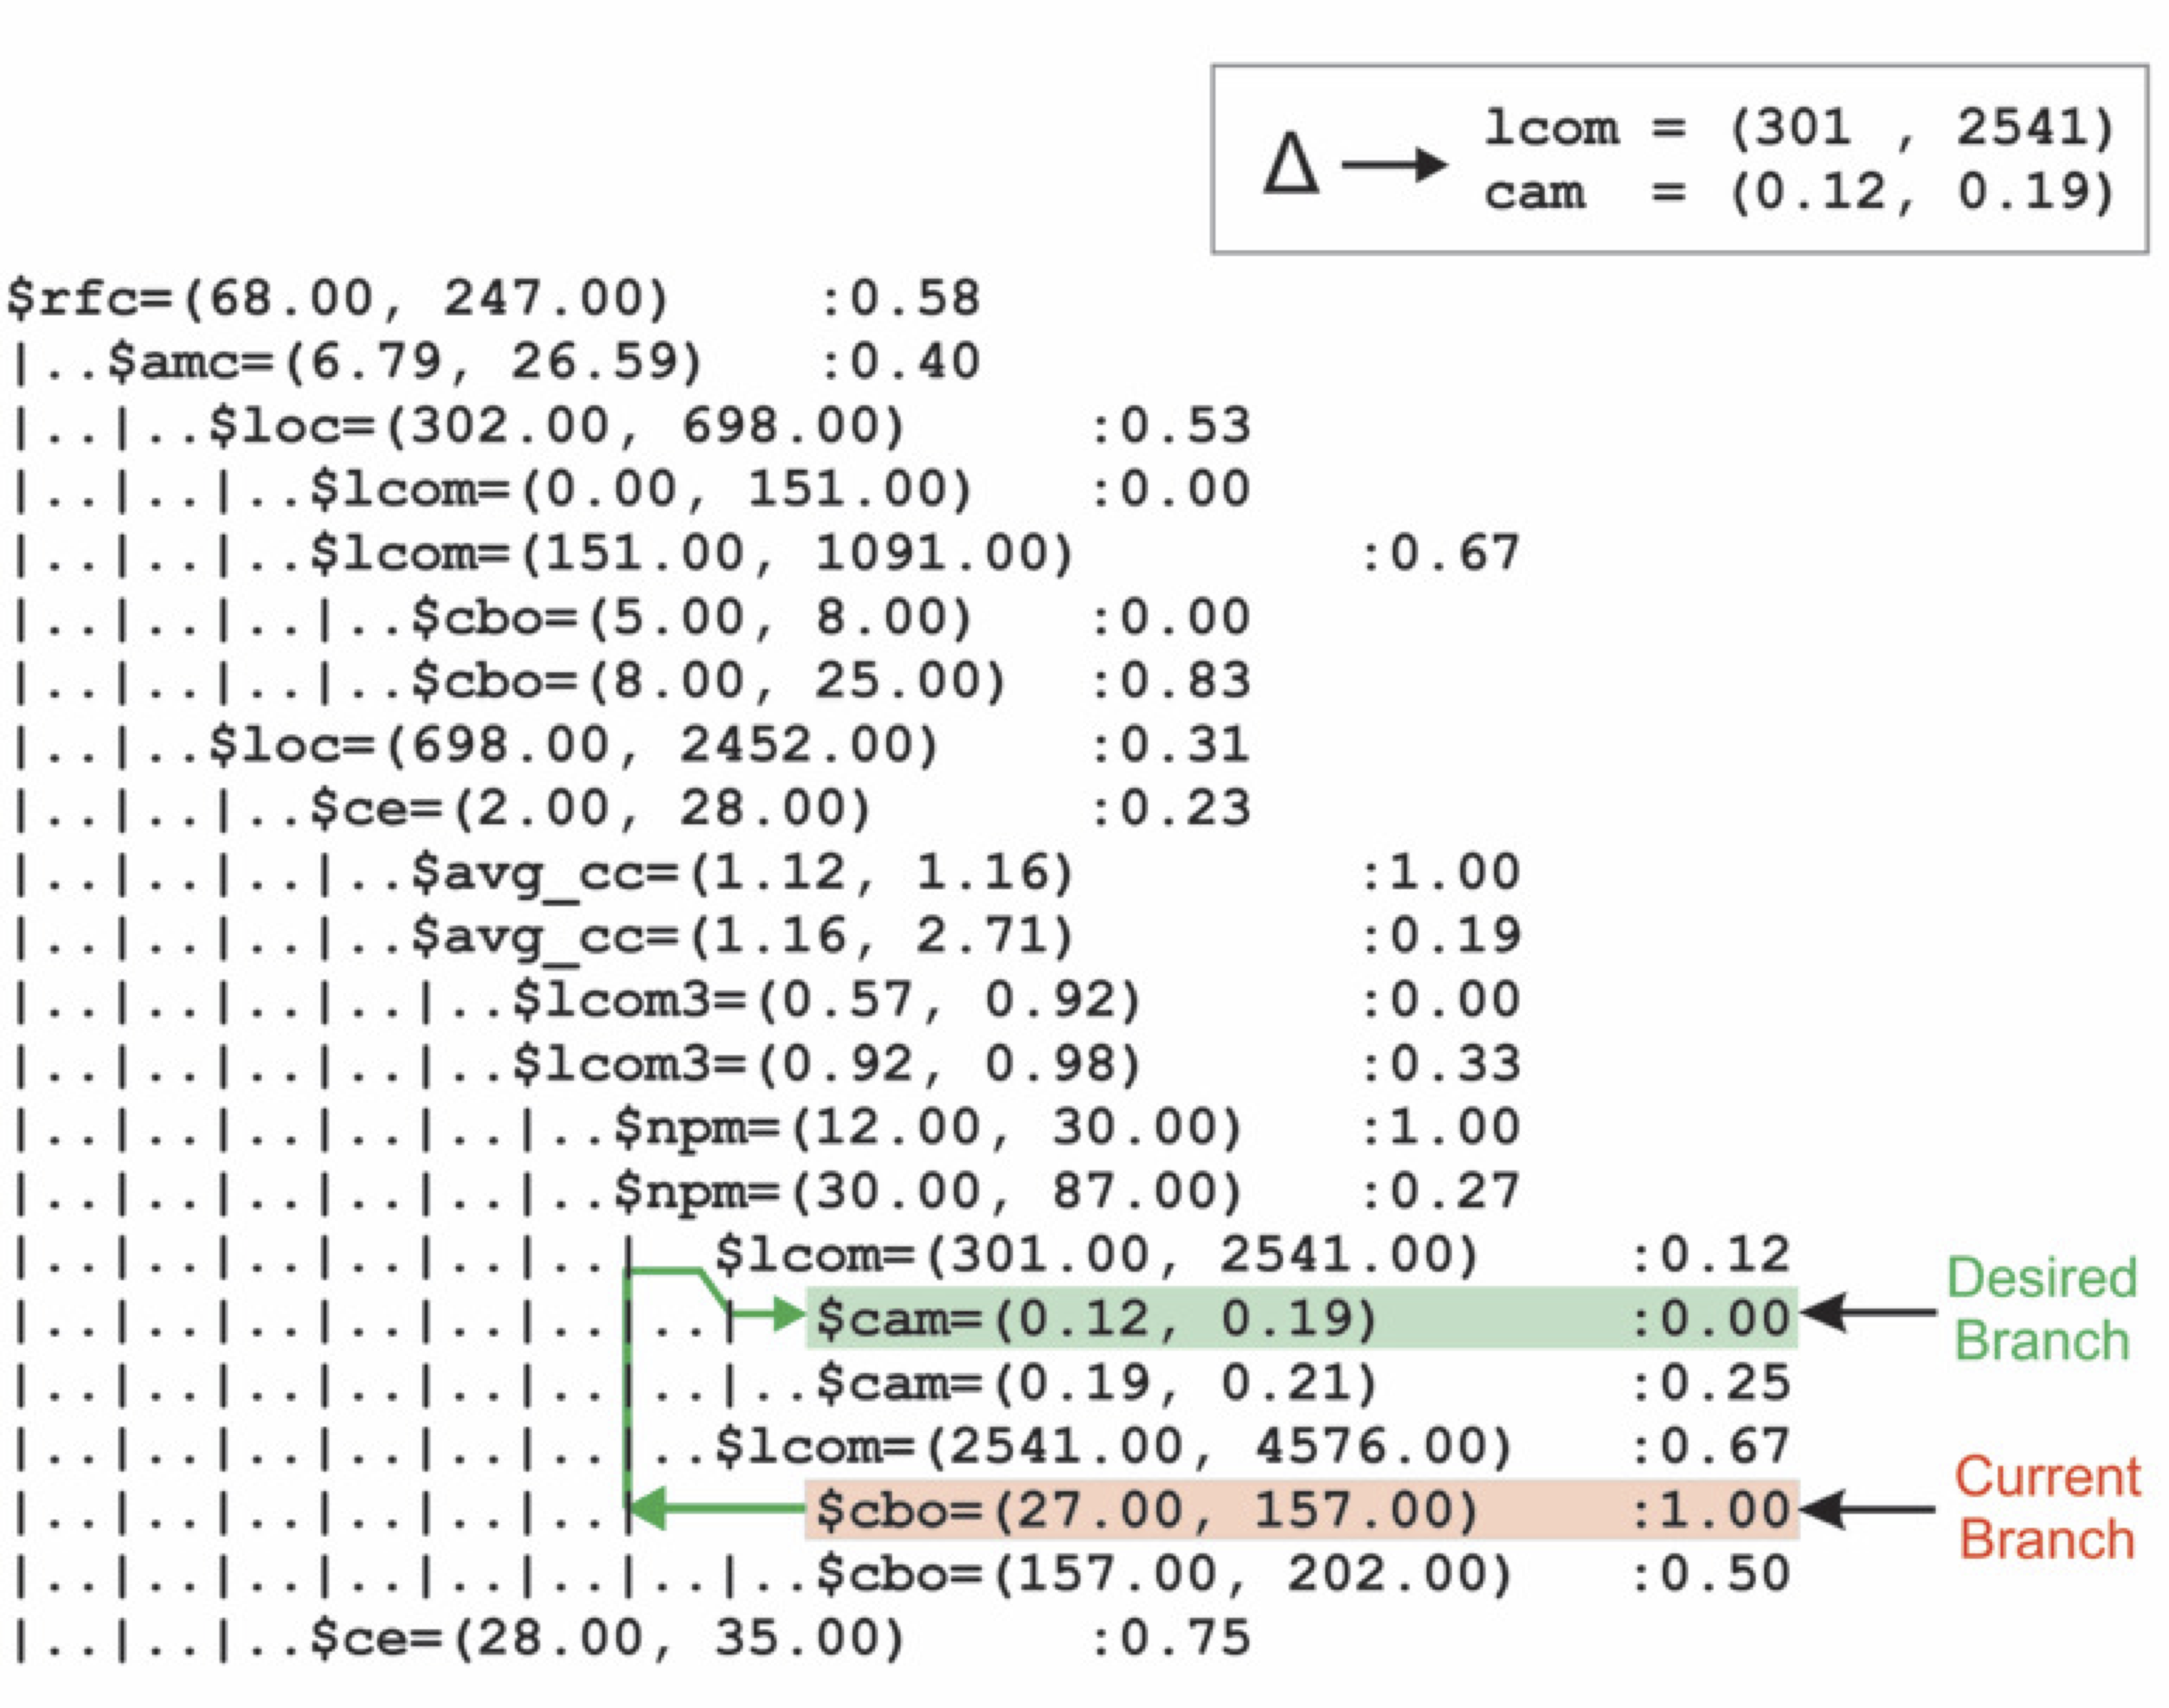
\includegraphics[width=0.8\linewidth]{XTREE_samp.png}
% ~\hrule~
\end{minipage}\bigstrut\\\hline
\\[-0.2cm]
\begin{minipage}{\linewidth}
\small
% \begin{shaded}  	   


{\bf \fig{xtree}.C: Using XTREE}

Using the training data,  divide the data using the decision tree algorithm of \fig{xtree}.A into groups of
size $\alpha=\sqrt{N}$.
For test item, 
	  find the {\em current } leaf: take each test instance, run it down to a leaf in the decision tree.  
After that,	  find the {\em desired} leaf:
		\begin{itemize}[leftmargin=3mm]
		\item Starting at {\em current}, ascend the tree $lvl\in \{0,1,2...\}$ levels;
		\item Identify {\em sibling} leaves; i.e. leaf clusters that can be reached from level $lvl$ that are not same as {\em current }
		\item Using the {\em score} defined above, find the {\em better} siblings; i.e. those with a {\em score} less than $\gamma=0.5$ times the mean score of {\em current}. 
		   If none found, then repeat for $lvl += 1$. Also,
		    return no plan if the new $lvl$ is above the root. 
		\item  Return the {\em closest} better sibling where distance is measured between the mean centroids of that sibling and {\em current}
		\end{itemize}
	 Also, find the {\em delta}; i.e. the set difference between  conditions in the decision tree branch to {\em desired} and {\em current}. To find that delta: (1)~for discrete attributes, delta is the value from {\em desired}; (2)~for  numerics, delta is the numeric difference; (3)~for numerics  discretized into ranges, delta is a random number selected from the low and high boundaries of the that range.
	 
		Finally, return the delta as the plan for improving the test instance.
% \end{shaded}
\end{minipage}\\\hline
\end{tabular}
\caption{Generating thresholds using XTREE.}\label{fig:xtree}
\end{figure*}